\documentclass{beamer}
\usepackage{graphicx}
\usepackage{caption}
\usepackage{multicol, multicolrule}
\SetMCRule{extend-fill=false}

\usetheme{CambridgeUS}
\usecolortheme{beaver}

\graphicspath{{./img}}

\title[PolyCooker]{PolyCooker - Présentation}
\author{Lucas Nouguier} 
\institute[]{Polytech Montpellier}
\date{02 Avril 2022}

\newcommand{\nologo}{\setbeamertemplate{logo}{}}
\AtBeginSection[]{
	\begin{frame}
		\frametitle{Sommaire}
		\tableofcontents[currentsection]
	\end{frame}
}

\logo{
\includegraphics[height=1.5cm]{LOGO_x1.png}}

\begin{document}

\frame{\titlepage}

\section{Contexte}
\begin{frame}
	\frametitle{Objectif}
	\centering
	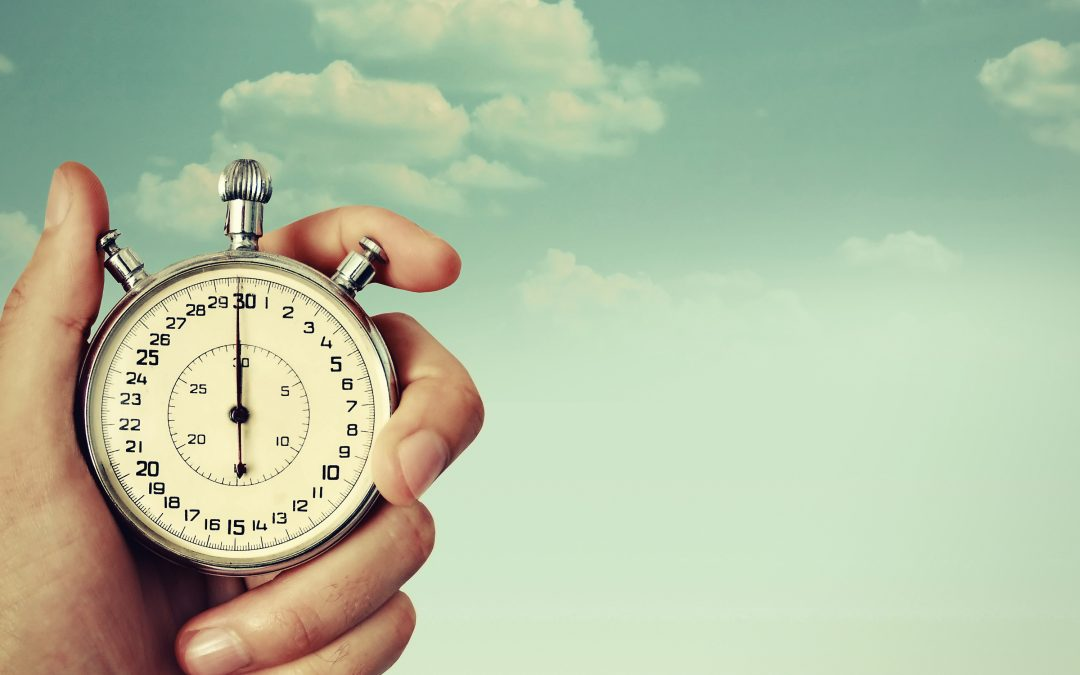
\includegraphics[height=0.6\textheight]{optiTemps.jpg}
\end{frame}

\begin{frame}
	\frametitle{Acteurs}
	\centering
	
\includegraphics[scale=0.5]{logoHommeFemme.png}
\end{frame}

\section{Aspect général \& fonctionnalités}
\begin{frame}
	\frametitle{Création de compte \& connexion}
	\begin{multicols}{2}
		\begin{figure}
			\centering
			\fbox{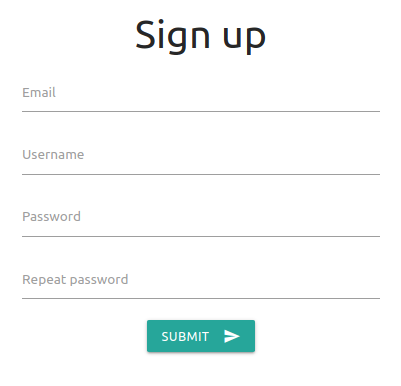
\includegraphics[width=0.9\linewidth]{signUp.png}}
			\caption{Création de compte}
		\end{figure}

		\columnbreak
		
		\begin{figure}
			\captionsetup{justification=raggedleft,singlelinecheck = false}
			\raggedleft
			\fbox{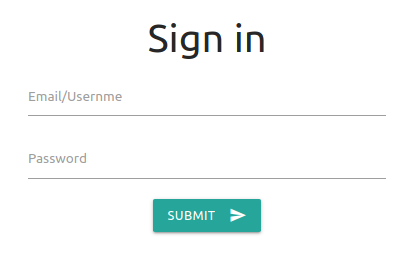
\includegraphics[width=0.6\linewidth]{signIn.png}}
			\caption{Connexion au compte}
		\end{figure}
		\captionsetup{justification=raggedright,singlelinecheck = false}
		\begin{figure}
			\raggedright
			\fbox{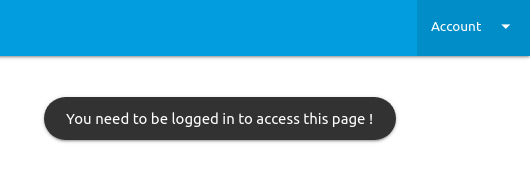
\includegraphics[width=0.6\linewidth]{error.png}}
			\caption{Toast d'erreur}
		\end{figure}
	\end{multicols}
\end{frame}

\begin{frame}
	\frametitle{Aspect}
	\begin{figure}
		\centering
		\fbox{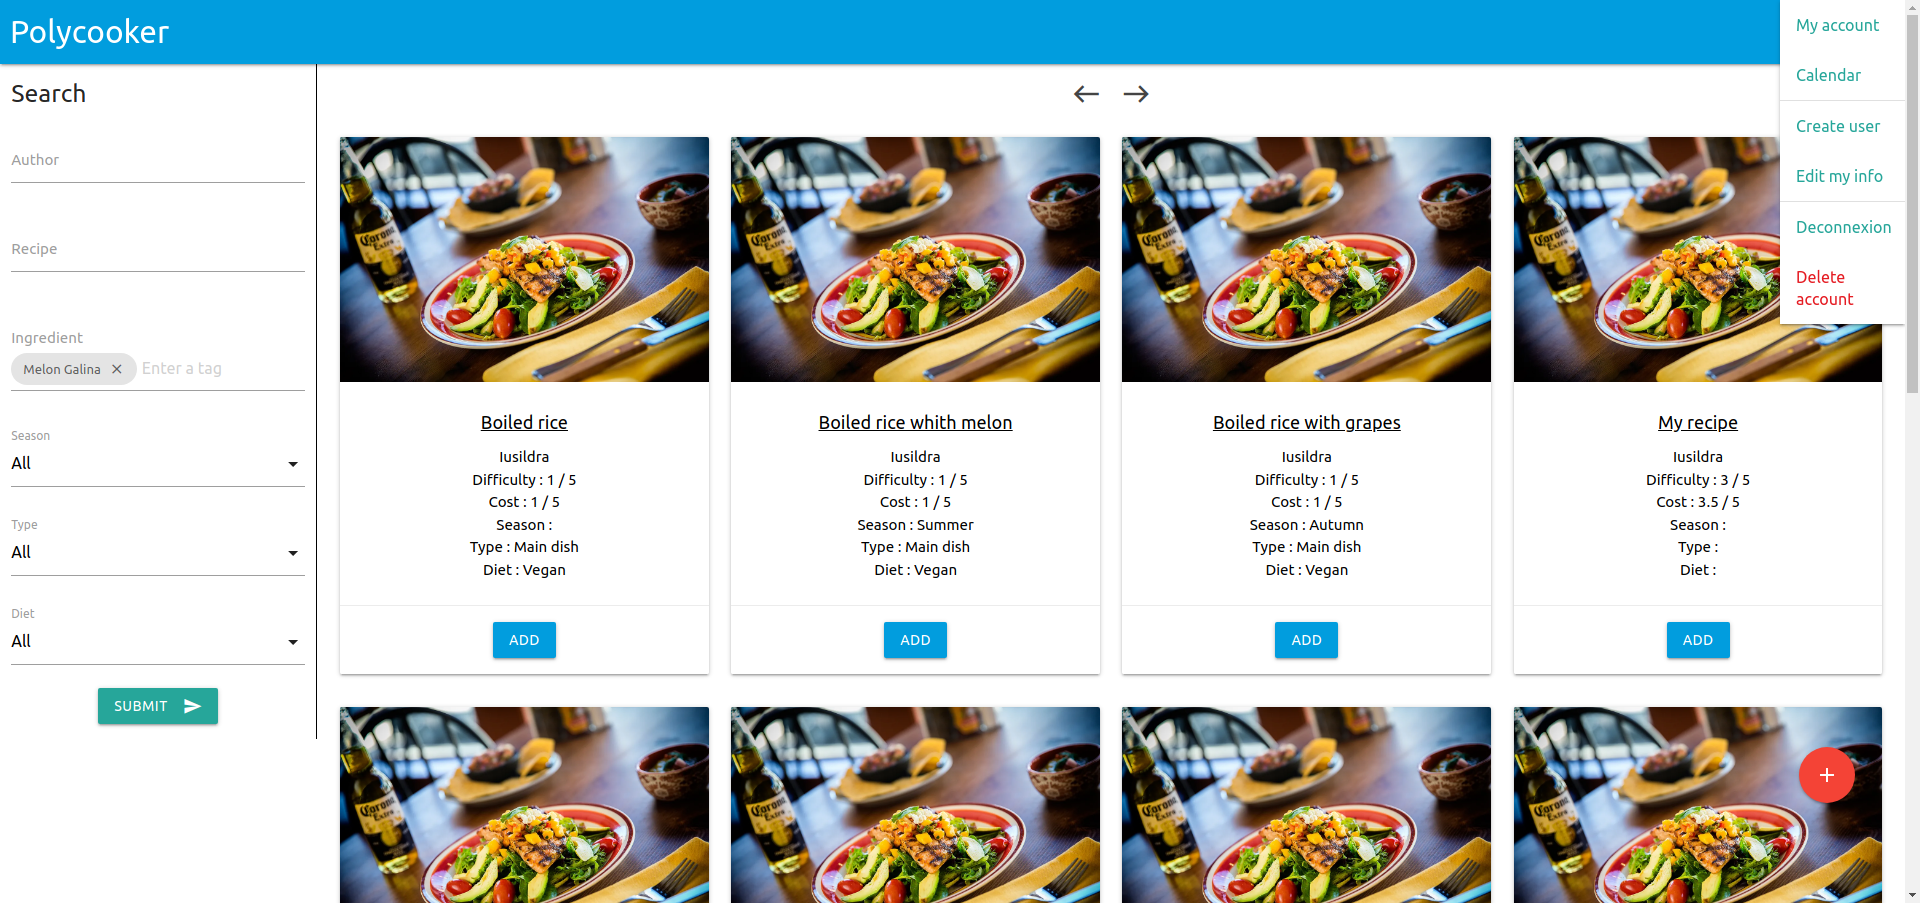
\includegraphics[width=0.9\linewidth]{homepage.png}}
		\caption{Page d'accueil de PolyCooker}
	\end{figure}
\end{frame}

\begin{frame}
	\frametitle{Fonctionnalités communes}
	\begin{multicols}{2}
		\begin{figure}
			\fbox{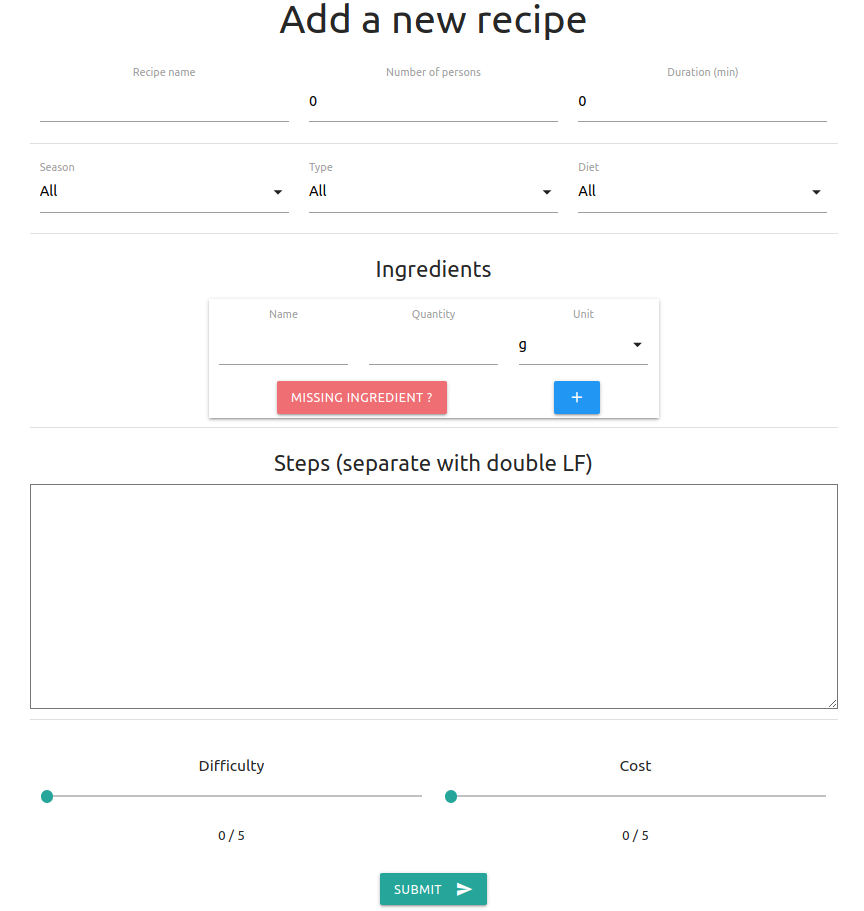
\includegraphics[height=0.6\textheight]{recipeCreation.png}}
			\caption{Création de recettes}
		\end{figure}
		
		\columnbreak
		
		\begin{figure}
			\raisebox{-0.25\textwidth}{
			\fbox{
			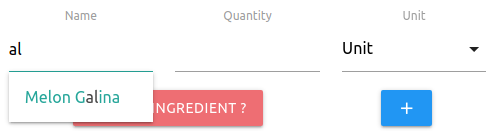
\includegraphics[width=0.85\linewidth]{addIngredient.png}}}
			\caption{Autocompletion}
		\end{figure}
	\end{multicols}
\end{frame}

\begin{frame}
	\frametitle{Fonctionnalités spécifiques}
	\begin{multicols}{2}
		\begin{figure}
			\fbox{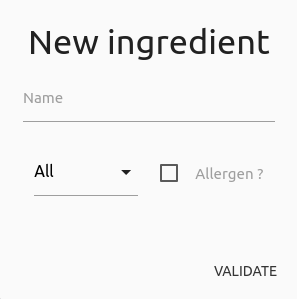
\includegraphics[width=0.4\linewidth]{createIngredient.png}}
			\caption{Création d'ingrédient}
		\end{figure}
		\begin{figure}
			\fbox{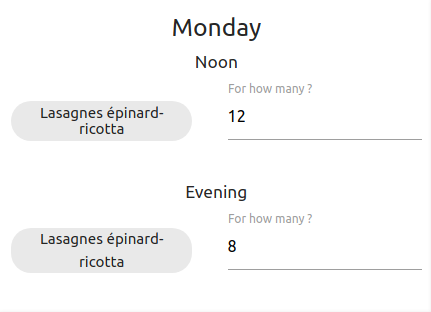
\includegraphics[width=0.4\linewidth]{calendar.png}}
			\caption{Prévision des repas}
		\end{figure}
		
		\columnbreak

		\begin{figure}
			\fbox{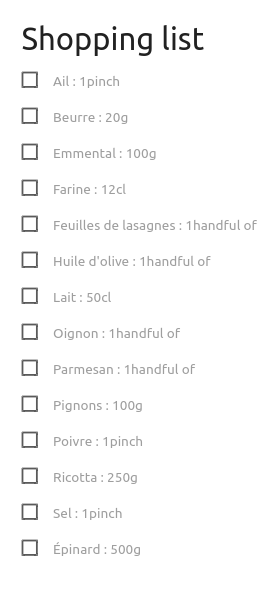
\includegraphics[height=0.55\textheight]{shoppingList.png}}
			\caption{Génération d'une\\liste de course}
		\end{figure}

	\end{multicols}
\end{frame}

\section{}

\nologo
    \begin{frame}
		\frametitle{Merci de votre attention}
		\vspace{-0.75cm}
		
\includegraphics[height=\textheight]{LOGO_x3.png}
		\centering
    \end{frame}

\end{document}